\section{Bayesian analysis}\label{sec:bayes}

\subsection{Model and exact marginal likelihood}
The Bayesian analysis uses the same Gaussian likelihood as Section~\ref{sec:freq} with priors on the signal parameters (Table~\ref{tab:priors}). The two linear amplitudes $a=a_c+ia_s$ get independent Gaussian priors, so that the SNR $\rho=|a|$ is Rayleigh$(\sigma_\rho)$; the default is $\sigma_\rho=10$.
With $z(\theta)=\sum_kX_kT_k^*e^{2\pi ik t_0}$ and $\rho^2(\theta)=|z|^2$ (the matched-filter output of the frequentist analysis at fixed $\theta=(t_0,f_0,Q)$) the integral over $a$ is a Gaussian integral:
\begin{equation}
\ln\frac{p(X|\theta,\mathcal M_1)}{p(X|\mathcal M_0)}=\frac12\frac{\sigma_\rho^2}{1+\sigma_\rho^2}\,\rho^2(\theta)-\ln(1+\sigma_\rho^2),\qquad
a\,|\,\theta,X\sim\mathcal N\!\Big(\tfrac{\sigma_\rho^2}{1+\sigma_\rho^2}z,\ \tfrac{\sigma_\rho^2}{1+\sigma_\rho^2}\Big).
\end{equation}
The closed form agrees with a brute-force two-dimensional integration over $a$ to $10^{-13}$ ($\ln B=10.7017$ both ways). The posterior of $\theta$ and the Bayes factor $B_{10}$ then need only the matched-filter cube $\rho^2(t_0,f_0,Q)$, i.e.\ exactly the object computed in Section~\ref{sec:freq}:
the two analyses differ only in how the cube is combined (maximum against prior-weighted average) and in the prior.

\begin{table}[h]\centering\small
\begin{tabular}{ll}
\toprule
parameter & prior\\
\midrule
$t_0$ & uniform on $[0.25,0.75]$\,s (as the injections)\\
$f_0$ & log-uniform on $[50,400]$\,Hz\\
$Q$ & uniform on $[4,15]$\\
$a_c,a_s$ & $\mathcal N(0,\sigma_\rho^2)$ each, $\sigma_\rho=10$\\
\bottomrule
\end{tabular}
\caption{Priors of the Bayesian analysis.}\label{tab:priors}
\end{table}

\subsection{Exact grid posterior and MCMC cross-check}
The posterior is evaluated exactly on a grid of $96$ log-spaced $f_0$ $\times$ $12$ values of $Q$ $\times$ $512$ time steps ($5.9\times10^5$ cells, uniform prior per cell by construction); the SNR posterior is the mixture over cells of Rice densities.
Figure~\ref{fig:post} shows one noise window with the same sine-Gaussian injected at $\snr=5,8,12,20$: at $\snr=5$ the $(f_0,Q)$ posterior is broad, from $\snr=8$ the time of arrival is determined to a millisecond and at $\snr\ge12$ everything collapses around the truth; the noise-only window gives a nearly flat $t_0$ posterior and an SNR posterior
piled up at small $\rho$ (the prior speaking).
An independent \texttt{emcee}~\cite{emcee} run (five parameters, no marginalisation, 40 walkers $\times$ 6000 steps) agrees with the grid on means and widths for $\snr=8,12,20$ (e.g.\ $f_0=151.9\pm2.4$ against $152.0\pm2.4$\,Hz at $\snr=8$); the integrated autocorrelation time is 260--380 steps (acceptance $0.32$--$0.38$),
i.e.\ 420--610 effective samples. One difference is informative: at $\snr=20$ the grid width of $f_0$ is $1.65$\,Hz against $1.14$\,Hz from MCMC, because the posterior is narrower than the grid cell (2.3\,\%, i.e.\ 3.4\,Hz); at high SNR the grid is the limiting factor.

\begin{figure}[h]\centering
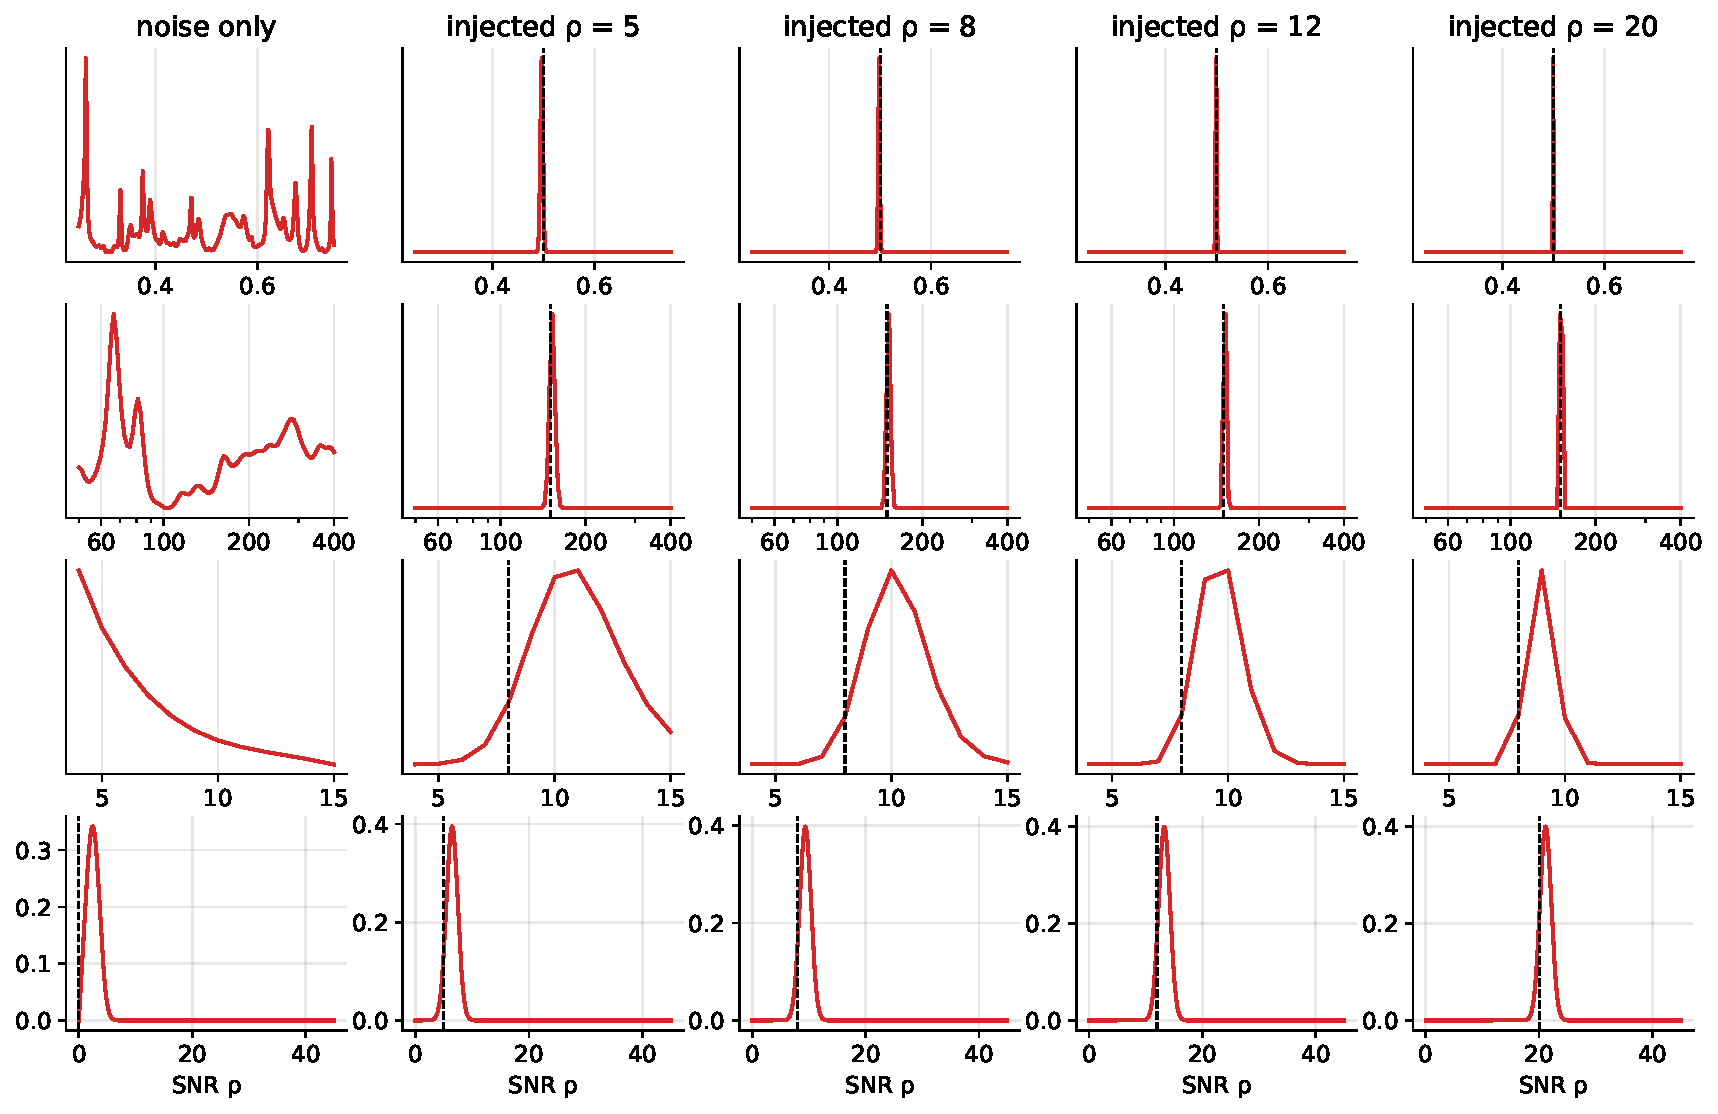
\includegraphics[width=0.95\textwidth]{fig04_posteriors.pdf}
\caption{Posterior marginals of $t_0$, $f_0$, $Q$ and $\rho$ for the same noise window with no signal and with a sine-Gaussian ($t_0=0.5$\,s, $f_0=150$\,Hz, $Q=8$) injected at $\snr=5,8,12,20$; dashed: truth.}\label{fig:post}
\end{figure}

\subsection{Bayes factor as a detection statistic}
We compute $\ln B_{10}$ with the same 160-template bank as the frequentist statistic, on the same background and injections. Three facts:
\begin{itemize}[nosep]
\item \textbf{On real noise the Bayes factor is not a false-alarm probability.} A fraction $1.2\,\%$ ($0.3\,\%$) of the training (test) noise windows has $B_{10}>10$ and $0.9\,\%$ ($0.17\,\%$) has $B_{10}>100$: glitches are evidence for \emph{something} that the Gaussian model can only call a burst. The Jeffreys scale~\cite{Jeffreys} is a scale of evidence within the model; the false-alarm probability has to be calibrated on background exactly as for the frequentist statistic.
\item \textbf{Same detection power.} At equal FAP ($10^{-2}$) the efficiencies of $\lmax$ and $\ln B_{10}$ coincide within $0.01$ at every SNR ($\varepsilon(\snr=6)=0.718$ against $0.714$, $\varepsilon(\snr=8)=0.994$ for both) and so do the ROC AUCs ($0.9763$ against $0.9769$ at $\snr=6$; $0.9968$ for both at $\snr=8$): the ranking of the windows is almost identical.
\item \textbf{The prior matters for $B_{10}$, not for the ranking.} At fixed data the Bayes factor falls as $-2\ln\sigma_\rho$ for large prior width (Occam penalty for a prior that wastes mass on SNRs the data exclude): for a noise window it decreases monotonically from $0$ to $-7$ between $\sigma_\rho\to0$ and $100$, for a signal it has a maximum at $\sigma_\rho$ of the order of the true SNR ($\approx5$ for $\snr=8$, $\approx10$ for $\snr=12$); the range of the $t_0$ prior shifts it by the logarithm of the volume ratio (Fig.~\ref{fig:prior}).
Whenever a Bayes factor is quoted the prior must be quoted with it.
\end{itemize}

\begin{figure}[h]\centering
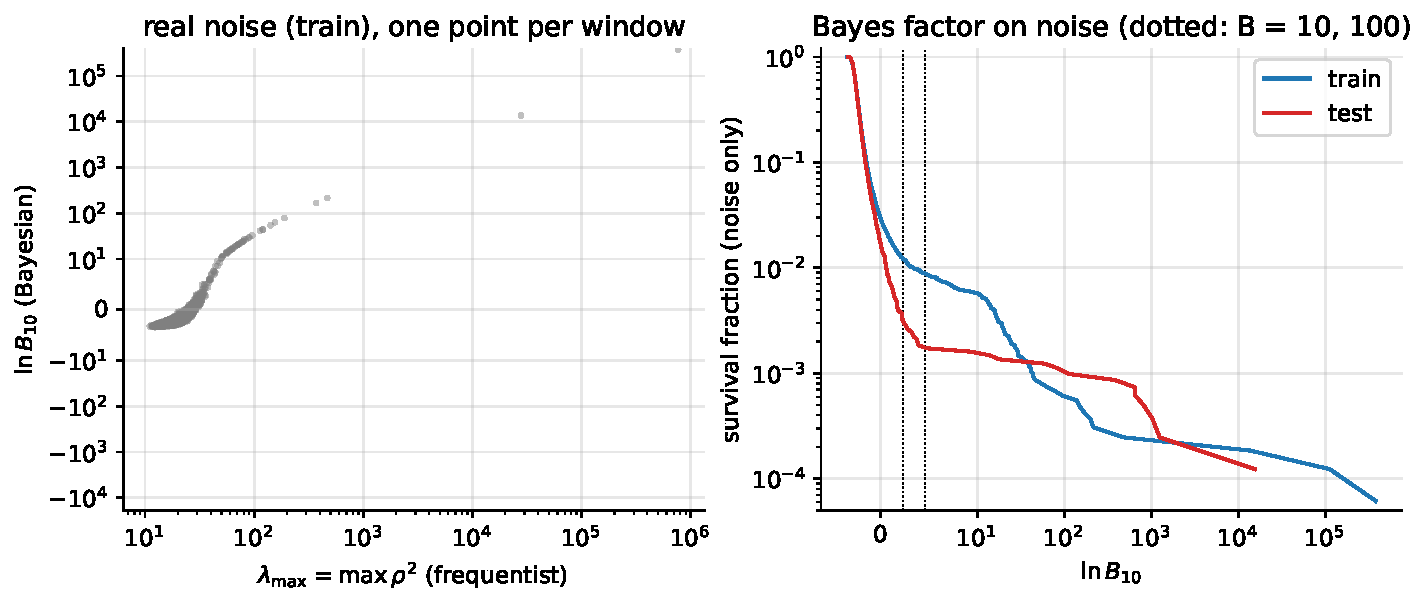
\includegraphics[width=0.48\textwidth]{fig04_bf_noise.pdf}\hfill
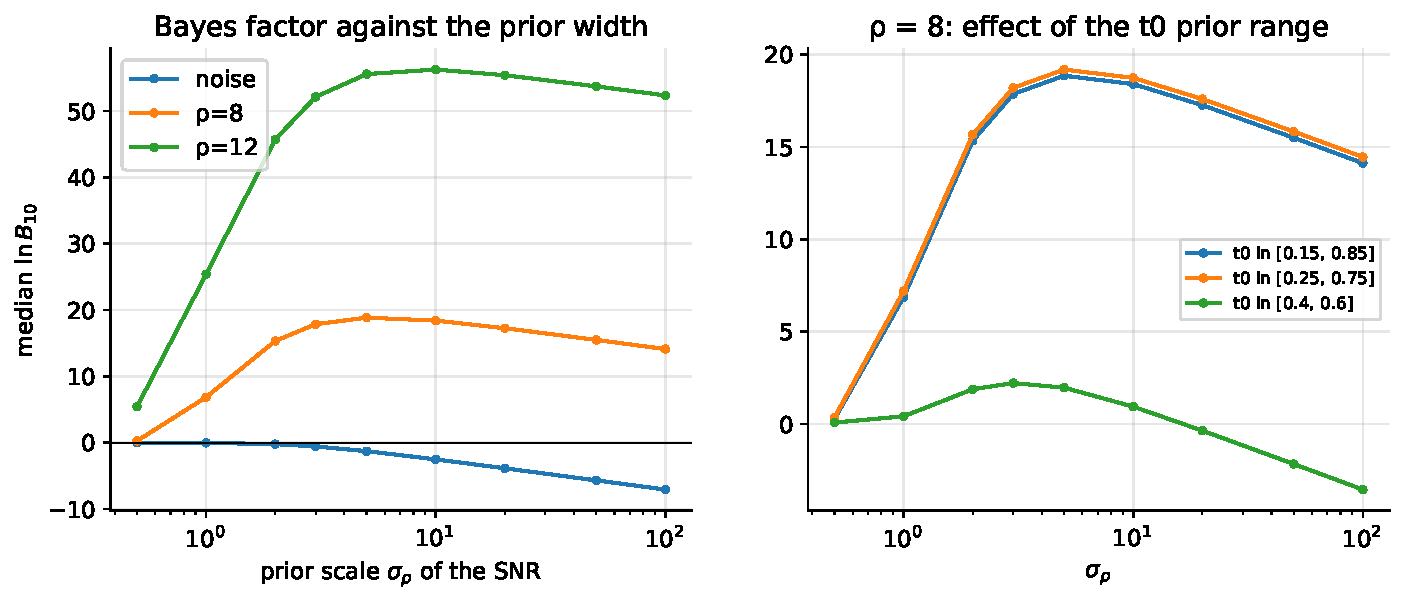
\includegraphics[width=0.48\textwidth]{fig04_prior_dependence.pdf}
\caption{Left: $\ln B_{10}$ against $\lmax$ on real noise (one point per window) and its tail. Right: median $\ln B_{10}$ against the prior width $\sigma_\rho$ for noise and sine-Gaussians at $\snr=8,12$; and for $\snr=8$ against the range of the $t_0$ prior.}\label{fig:prior}
\end{figure}

\subsection{Calibration of the posterior}
Simulation-based calibration~\cite{SBC} draws the truth from the prior, simulates data, and checks that the posterior CDF of the truth is uniform. With $500$ simulations in ideal Gaussian noise and $500$ in real test windows,
the rank histograms of $t_0$, $f_0$, $Q$ and $\rho$ are consistent with uniformity in both (Kolmogorov--Smirnov $p=0.24$--$0.90$ in Gaussian noise, $0.25$--$0.85$ in real noise), so that waveforms, whitening convention, closed-form marginalisation and grid are correct end to end. Five hundred simulations are too few to see an effect of the glitches ($\lesssim1\,\%$ of windows).
The coverage of the nominal 68\,\% credible intervals is $0.65$--$0.69$ for $Q$ and $\rho$ but $0.50$--$0.51$ for $f_0$ and $0.58$--$0.60$ for $t_0$, in both noises: this is a grid-resolution effect (for loud injections the posterior is narrower than a cell: $3.4$\,Hz in $f_0$, 1\,ms in $t_0$), not a model failure, and the MCMC does not have it.
A posterior-predictive check on the residual of the fit ($400$ injections at $\snr=10$) gives $0.25\,\%$ of p-values below $0.01$ and $2\,\%$ below $0.05$ (median $0.69$ instead of $0.5$, because the in-band noise variance is $1.975$ rather than $2$ per component).

\begin{figure}[h]\centering
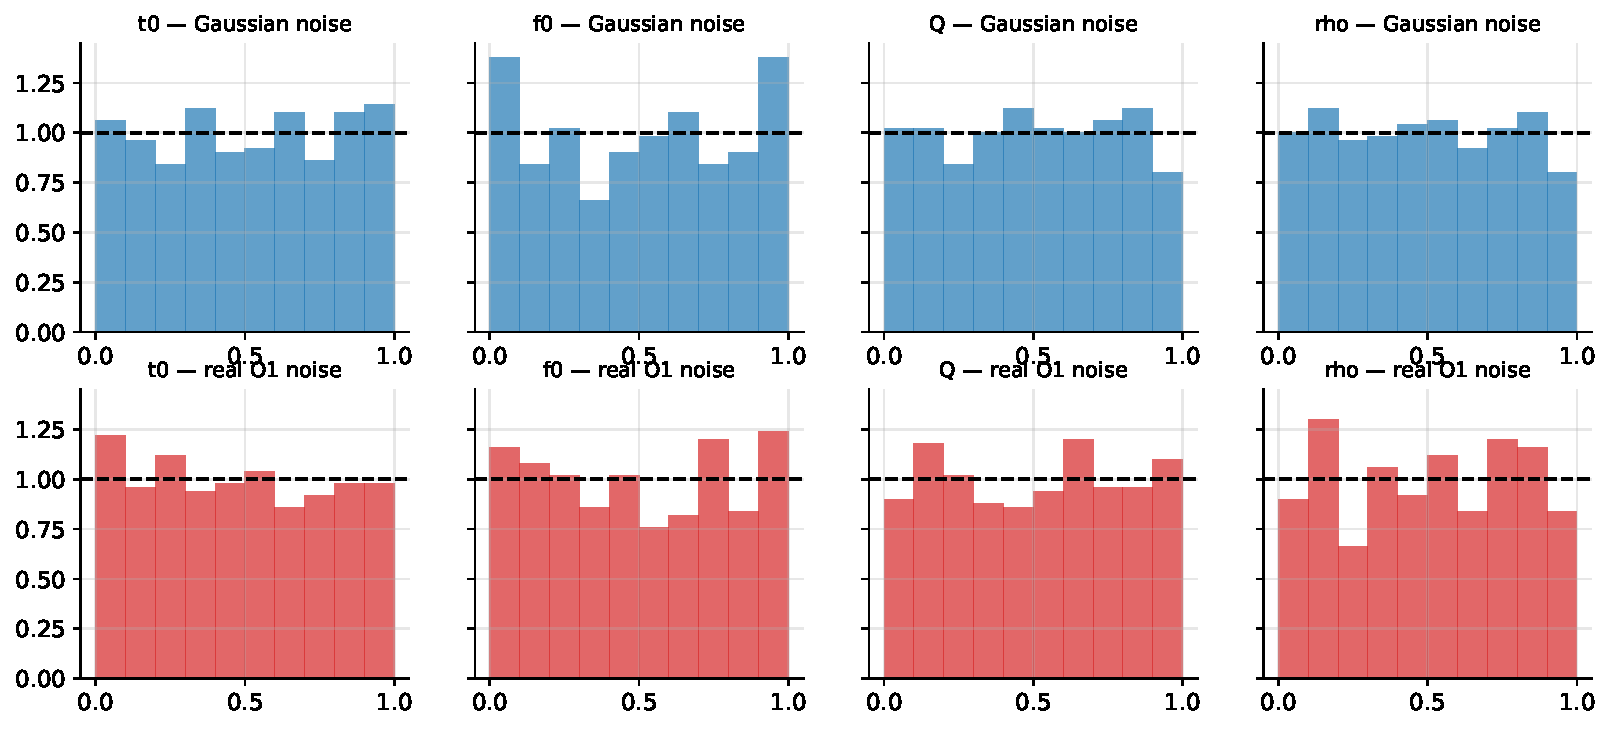
\includegraphics[width=0.95\textwidth]{fig04_sbc.pdf}
\caption{Simulation-based calibration: distribution of the posterior CDF of the true parameters (top: Gaussian noise; bottom: real O1 noise). Uniform = calibrated.}\label{fig:sbc}
\end{figure}

\subsection{Credible against confidence intervals at low SNR}
In the simplest setting where the two can be compared exactly (known template, $s\ge0$ measured through $\hat s=|z|$) we compute the frequentist coverage of the 68\,\% credible intervals by integrating the Rice density (Fig.~\ref{fig:cred}). For $s\gtrsim3$ credible and confidence intervals coincide at $68$--$69\,\%$
(the posterior becomes Gaussian and the prior irrelevant). Below that, credible intervals --- which are conditional on the observed data and make no coverage promise --- behave differently: with a flat prior the central interval covers $0$ at $s=0$, the HPD interval $77\,\%$ at $s=0$ and $85\,\%$ near $s=1$ before dipping to $53\,\%$ at $s\approx1.7$; with the Rayleigh$(10)$ prior both under-cover for $s\lesssim1.5$ ($54$--$60\,\%$ at $s=1$) because the prior prefers larger SNRs than the truth.
The Neyman/Feldman--Cousins intervals cover by construction, and the profile-likelihood interval lies in between ($39\,\%$ at $s=0$, $74\,\%$ at $s=1$). The HPD intervals are shorter than the profile ones for $\hat s\lesssim2$: informativeness is traded against guaranteed coverage.

\begin{figure}[h]\centering
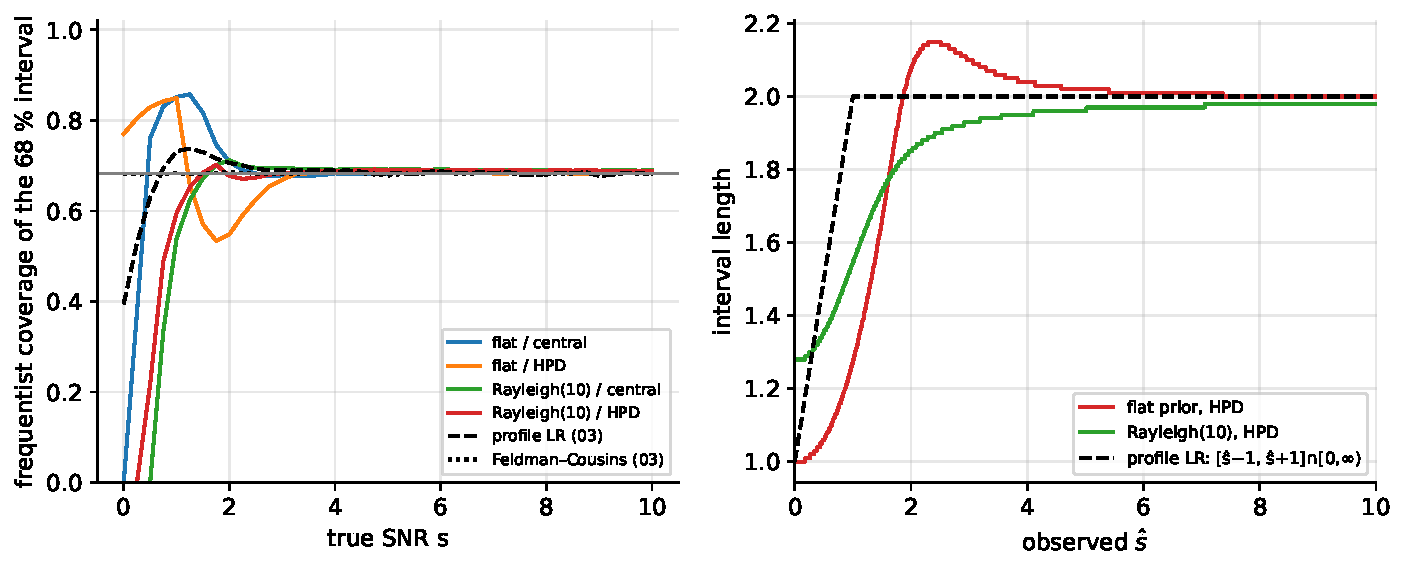
\includegraphics[width=0.95\textwidth]{fig04_credible_vs_confidence.pdf}
\caption{Left: frequentist coverage of the nominal 68\,\% intervals against the true SNR (credible intervals with two priors and two orderings; profile likelihood and Feldman--Cousins from Section~\ref{sec:freq}). Right: interval length against the observed $\hat s$.}\label{fig:cred}
\end{figure}

\subsection{Labelled glitches and a glitch-aware Bayes factor}\label{sec:glitchbayes}
Real glitches have no labels, so notebook~21 injects three labelled families into real test noise: blips (one-sided decaying sinusoids), whistles (fast sweeps, $1500$--$5000\,$Hz/s) and scattered-light-like arches, scaled to a given norm $\rho$ of the whitened bins. At the FAP $10^{-2}$ thresholds of the validation noise and $\rho=8$ (Fig.~\ref{fig:glitchdisc}) the bank, the Bayes factor and the CNN alarm on $97$--$98\,\%$ of the blips (a blip is a low-$Q$ sine-Gaussian: a single detector cannot tell them apart) and on $38$--$53\,\%$ of whistles and arches, which the sine-Gaussian templates fit poorly; the mean alarm fraction on glitches grows from $0.06$ ($\rho=4$) to $0.97$ ($\rho=14$) for the bank, and the Allen $\chi^2$ test removes only $\approx25\,\%$ of the alarms at $\rho=14$ while it also rejects $12\,\%$ of loud real signals. A $\chi^2$ test is not a glitch veto against glitches that fit a template well.

A \emph{glitch-aware} Bayes factor treats the noise hypothesis as ``Gaussian noise or one of the three glitch families'' with prior weight $\eta=0.1$ for the glitch, using a $51$-template glitch bank and the same analytic amplitude marginalisation ($\sigma_\rho=10$): $\ln B_{\rm rob}=\ln B-\ln[(1-\eta)+\eta B_{\rm glitch}]$. At $\rho=8$ it lowers the alarm rate on blips from $0.97$ to $0.35$, on whistles from $0.38$ to $0.04$ and on arches from $0.52$ to $0.19$, at the cost of the efficiency for real signals ($0.88$ against $0.96$ mean over the three morphologies at $\rho=8$; $0.78$ against $0.99$ for pulses, which resemble blips). The AUC of signal against glitch among the alarms rises from $0.52$ to $0.87$ (blips) and from $0.93$ to $0.97$ (whistles). On the \emph{real} noise windows the fraction with $B>100$ only goes from $0.17\,\%$ to $0.15\,\%$ (test) and from $0.21\,\%$ to $0.18\,\%$ (validation): the false $B>100$ of Section~\ref{sec:bayes} are not made of glitches of these three families. The gain is an upper bound for unseen glitch types, because the glitch model contains the families that were injected.
\begin{figure}[h]\centering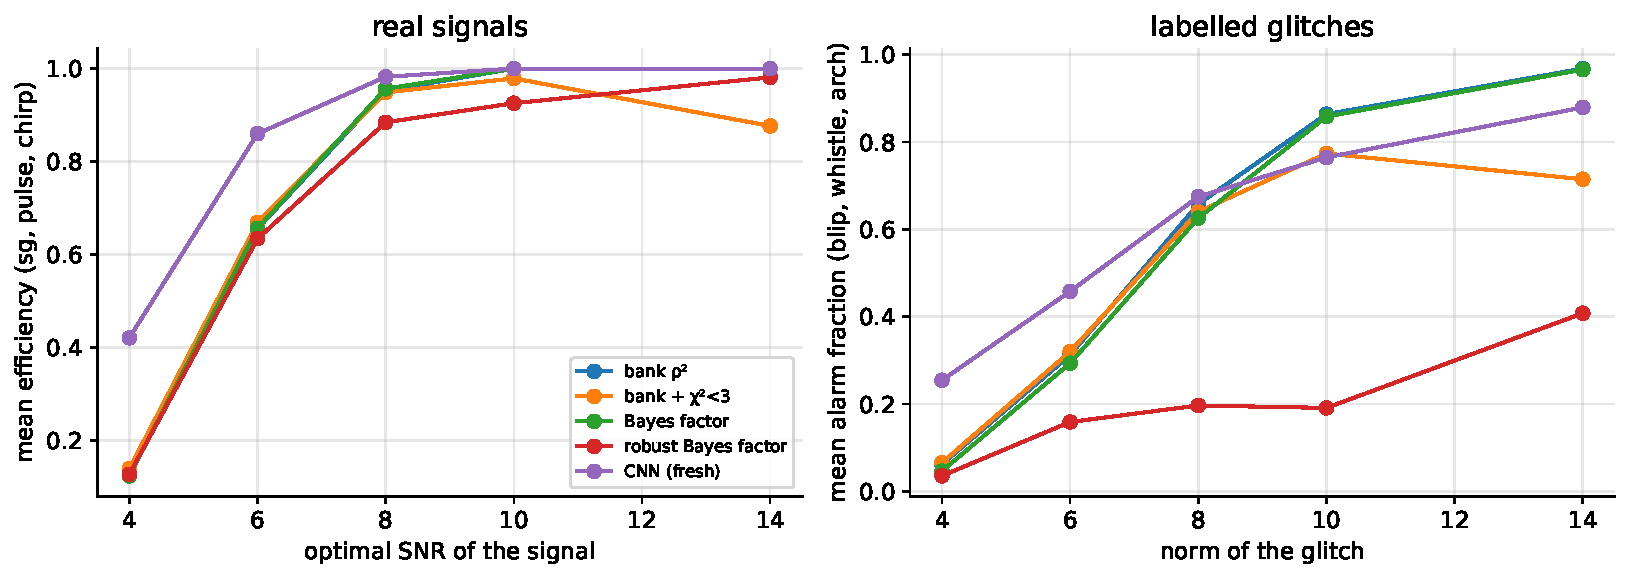
\includegraphics[width=0.95\textwidth]{fig21_glitch_discrimination.pdf}\caption{Alarm fraction at FAP $10^{-2}$ against the norm, for real signals (left, mean of sine-Gaussian, pulse, chirp) and for the labelled glitches (right).}\label{fig:glitchdisc}\end{figure}

\subsection{Exact-model MCMC, two-detector evidence and calibration}\label{sec:bayesext}
\paragraph{Exact IMRPhenomD model (notebook~32).} For the dominant mode a detector sees $\mathrm{Re}[C\,h(f)]$ with one complex constant $C$ (distance, inclination, polarisation, antenna pattern and phase), so with a Gaussian prior on $C$ the likelihood of the aligned-spin IMRPhenomD model is analytic and only $(M,q,\chi_1,\chi_2,t_{\rm merge})$ are sampled ($32$ walkers $\times1500$ steps of \texttt{emcee}, $\approx1$\,ms per likelihood; autocorrelation time $\approx117$ steps, i.e.\ $\approx270$ independent samples per chain). On $30$ injections per SNR the median error of $M_c$ is $4.7$, $6.3$, $6.8\,\%$ at $\snr=8,12,16$, of $M$ $5.1$, $7.9$, $5.3\,\%$, of $q$ $22$--$28\,\%$, of $\chi_{\rm eff}$ $0.13$, $0.09$, $0.06$ and of the merger time $1$--$2\,$ms, with $68\,\%$ interval coverage of $0.67$--$0.83$ for $M_c$, $0.60$--$0.70$ for $q$, $0.67$--$0.73$ for $\chi_{\rm eff}$ and $0.43$--$0.70$ for $M$ ($\pm0.09$ from $30$ injections; the merger time, whose width is $2$--$4\,$ms, has $0.5$ because of the $\sim$ms offset between the template and the envelope peak that defines the injected time). The accuracy is the same as that of the non-spinning grid ($\approx7\,\%$, Section~\ref{sec:pe}): the spin and mass-ratio degeneracies, not the model, limit $M_c$ and $M$; but the intervals are calibrated, while those of the grid posterior covered the truth only in $9$--$32\,\%$ of the cases.
\paragraph{Signal or glitch with two detectors.} Bayes factors with amplitude marginalisation ($\sigma=10$) of a coherent signal (one complex amplitude, real detector weights integrated over the angle), of a glitch in H1 only or in L1 only (equal prior) and of independent signals, evaluated at the peak of each template, are used to classify physical network injections against blips in one detector of the same network norm. The AUC of the odds $\ln B_C-\ln B_G$ is $0.72$, $0.85$, $0.91$, $0.93$ at network norm $6,8,10,12$, no better than that of $\min(\rho_H^2,\rho_L^2)$ ($0.74$, $0.87$, $0.92$, $0.94$): with two detectors almost all the discrimination comes from requiring a signal in both. The odds are \emph{not} calibrated: a $\ln B_C-\ln B_G>\ln100$ occurs in $8\,\%$ of the noise window pairs ($32\,\%$ for $\ln B_C$ alone), because the profile over $24$ templates and the lag peaks is not the marginalisation of Section~\ref{sec:bayes} and carries the full look-elsewhere factor; its threshold must be set on the background, as for any frequentist statistic.
\paragraph{Simulation-based calibration of the grid posterior.} In Gaussian noise, with data drawn from the generative model ($1500$ simulations), the posterior of $(f_0,Q,t_0)$ over the sine-Gaussian bank is close to calibrated but not exactly: the Kolmogorov--Smirnov distance of the rank from the uniform is $0.05$--$0.06$ for $f_0$ and $Q$ and $0.16$--$0.18$ for $t_0$ (mean rank $0.61$: the posterior sits $\approx$ half a lag-bin early; $\mathrm{KS}\,p<10^{-3}$ for all with this many simulations), and the central $68\,\%$ interval contains $71$--$74\,\%$ of the truths for $f_0$ and $Q$. A four times finer grid ($640$ against $160$ templates) does not improve it ($0.060$ against $0.050$ for $f_0$): the residual is the discretisation of the lag and of the template cells, not the density of the bank.
\begin{figure}[h]\centering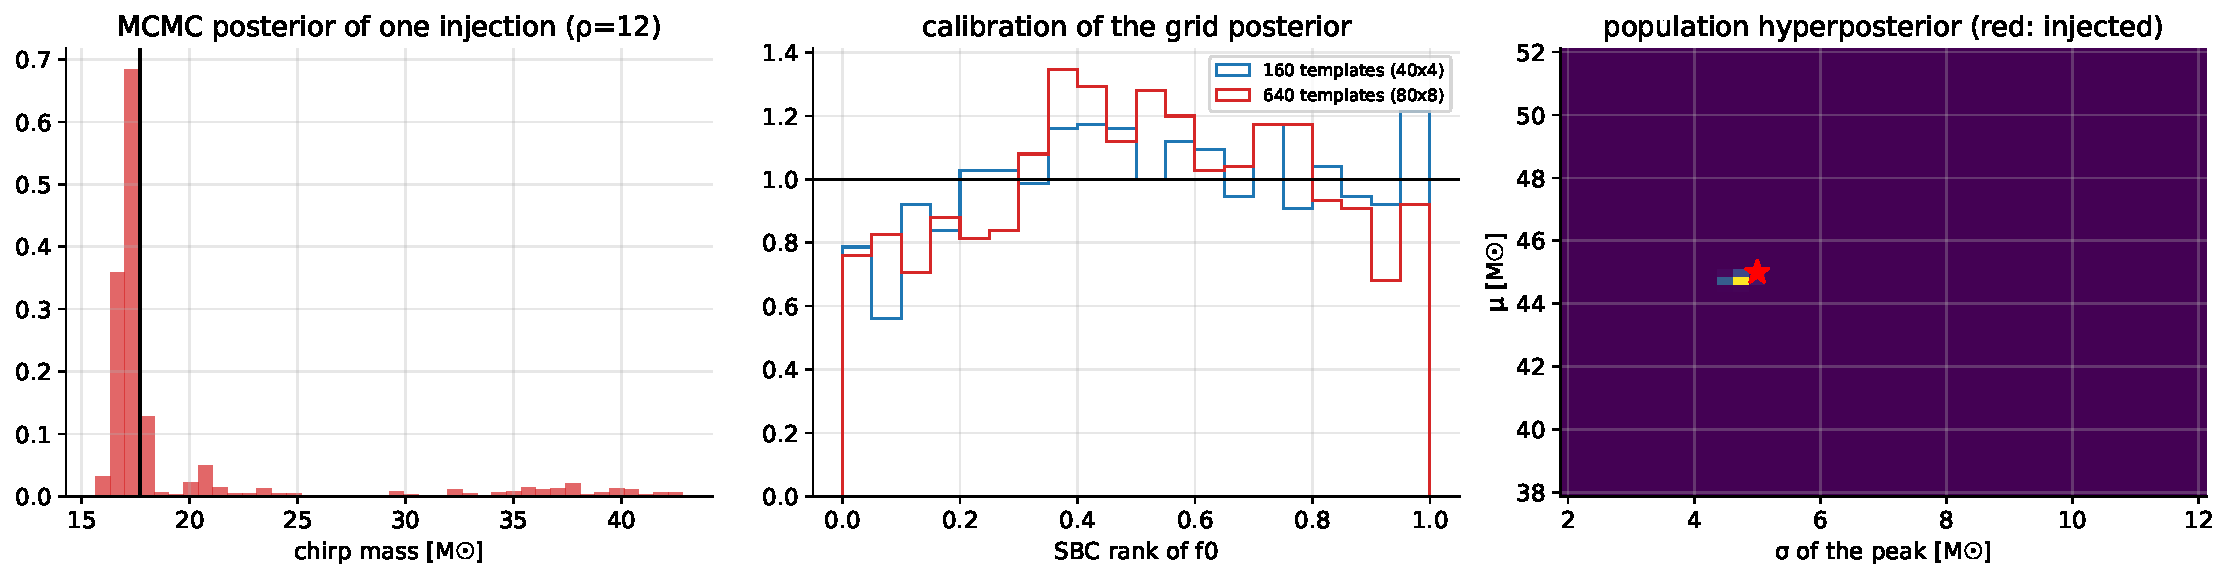
\includegraphics[width=0.98\textwidth]{fig32_bayes_extensions.pdf}\caption{Left: MCMC posterior of the chirp mass of one injection. Centre: SBC rank of $f_0$ for the two banks. Right: hyperposterior of the mass distribution of Section~\ref{sec:unfold}.}\label{fig:bayesext}\end{figure}
